\documentclass[11pt]{article}
\usepackage[margin=1in]{geometry}
\usepackage{amsmath,amssymb}
\usepackage{algorithm}
\usepackage{algpseudocode}
\usepackage{tikz}
\usetikzlibrary{automata,positioning,arrows.meta}
\usepackage{graphicx}
\usepackage{fancyhdr}
\usepackage{enumerate}
\usepackage[colorlinks=true,linkcolor=blue,urlcolor=blue]{hyperref}

\newcommand{\hwnum}{5}

% page header, same as the posted solutions
\pagestyle{fancy}
\fancyhf{}
\lhead{EECS 376: Foundations of Computer Science\\University of Michigan, Fall 2026}
\rhead{\vspace{\baselineskip}Solutions to Homework \hwnum}
\cfoot{\thepage}
\setlength{\headheight}{28pt}

% pseudocode labels
\renewcommand{\algorithmicrequire}{\textbf{Input:}}
\renewcommand{\algorithmicensure}{\textbf{Output:}}

% notation
\newcommand{\set}[1]{\left\{#1\right\}}
\newcommand{\abs}[1]{\left|#1\right|}
\newcommand{\floor}[1]{\left\lfloor #1 \right\rfloor}
\newcommand{\ceil}[1]{\left\lceil #1 \right\rceil}
\newcommand{\inner}[1]{\langle #1 \rangle}
\newcommand{\algo}[1]{\textsc{#1}}
\newcommand{\OPT}{\mathrm{OPT}}
\newcommand{\ALG}{\mathrm{ALG}}

% automata style
\tikzset{
  every state/.style={minimum size=22pt,inner sep=1pt,font=\small},
  >=Stealth,
  initial text=start,
}

% one part per page for Gradescope
\newcommand{\qpage}[1]{\clearpage\noindent\textbf{\large #1}\par\medskip}

\begin{document}

\noindent\textbf{\large Q0 Before you start; before you submit}\par\medskip

I did not collaborate with anyone on this homework.

\qpage{Q1 Self assessment}

The part of HW4 with the most room for improvement is Question 3(b), the exchange argument for the greedy refueling algorithm.
My answer was correct, but it was much longer and harder to read than the posted one.
Here is the middle of what I submitted, after I defined $j$ as the first town of $\OPT$ after $a = i_{\text{diff}-1}$ and set $\OPT' = (\OPT \setminus \set{j}) \cup \set{i_{\text{diff}}}$:

\begin{quote}\small\emph{
$\OPT'$ is valid.
Let $p < q$ be two consecutive elements of $\set{0} \cup \OPT' \cup \set{n}$; I show $\mathrm{dist}(p,q) \le R$.
Note that $i_{\text{diff}} \in \OPT'$, so it is impossible that $p < i_{\text{diff}} < q$.
That leaves two cases.
Case $q \le i_{\text{diff}}$. The town $a$ is in $\set{0}\cup\OPT'$ \ldots, so $a < q$.
Since $p$ is the element right before $q$, we get $p \ge a$. So $a \le p < q \le i_{\text{diff}}$, and by Facts 1 and 2, $\mathrm{dist}(p,q) \le \mathrm{dist}(a,i_{\text{diff}}) \le R$.
Case $p \ge i_{\text{diff}}$. Above $i_{\text{diff}}$, the sets $\OPT$ and $\OPT'$ agree \ldots
If $p > i_{\text{diff}}$, then $p$ and $q$ are also consecutive in $\set{0}\cup\OPT\cup\set{n}$ \ldots
If $p = i_{\text{diff}}$, then $q$ is the smallest element of $\OPT' \cup \set{n}$ above $i_{\text{diff}}$ \ldots
Let $p'$ be the element of $\set{0}\cup\OPT$ right before $q$ \ldots so $p' < i_{\text{diff}}$ \ldots
Fact 1 gives $\mathrm{dist}(i_{\text{diff}},q) \le \mathrm{dist}(p',q) \le R$.}
\end{quote}

What was deficient: the logic is sound, but the organization is bad.
I proved validity by taking an arbitrary pair of consecutive stops $p < q$ in $\OPT'$ and splitting into cases on where the pair sits relative to $i_{\text{diff}}$.
That forces the reader to track two helper facts, three cases, and extra names like $p'$, just to check something that has a two-line explanation.
A grader would have a hard time finding the three things that actually matter.

How to fix it: the posted solution organizes the same argument around the stretches of $\OPT'$ instead of around arbitrary pairs.
There are only three kinds of stretches.
(1) Every stretch up to and including the one that ends at $i_{\text{diff}}$ lies inside a stretch that the greedy algorithm drove on one pack, so it has distance at most $R$.
(2) The stretch leaving $i_{\text{diff}}$ ends at the next stop of $\OPT$ and starts later than $\OPT$'s own stretch into that stop (because $j < i_{\text{diff}}$), so it is shorter than a stretch of $\OPT$, hence at most $R$.
(3) Every stretch after that is unchanged from $\OPT$.
Writing it this way, the proof fits in one short paragraph, and each sentence corresponds directly to one rubric item (the stretches into $i_{\text{diff}}$, the stretch out of $i_{\text{diff}}$, and the rest).
Next time I will first identify what actually changes between $\OPT$ and $\OPT'$ and only argue about those parts, instead of re-checking everything from scratch.

\qpage{Q2.1 Keeping things fresh with potpourri (a)}

\textbf{Recurrence.}
For $n \le 2$ the function does a constant amount of work (one comparison and possibly a swap), so $T(1) = T(2) = \Theta(1)$.
For $n > 2$ it computes $t = \ceil{2n/3}$, makes three recursive calls on subarrays of size $t$, and does nothing else.
Passing a subarray is just passing two indices, so the work outside the recursive calls is $\Theta(1)$.
Ignoring the ceiling, as allowed,
\[
  T(n) = 3\,T\!\left(\tfrac{2n}{3}\right) + \Theta(1) \qquad (n > 2), \qquad T(1) = T(2) = \Theta(1).
\]

\textbf{Master Theorem.}
Here $a = 3$, $b = 3/2$, and $f(n) = \Theta(1) = \Theta(n^0)$.
The critical exponent is
\[
  \log_b a = \log_{3/2} 3 = \frac{\ln 3}{\ln (3/2)} \approx 2.71 .
\]
Since $f(n) = O(n^{\log_b a - \varepsilon})$ for, say, $\varepsilon = 1$, we are in the first case of the Master Theorem (the leaves dominate), and
\[
  T(n) = \Theta\!\left(n^{\log_{3/2} 3}\right) \approx \Theta(n^{2.71}).
\]
So \algo{StoogeSort} is slower than even insertion sort.

\qpage{Q2.2 Keeping things fresh with potpourri (b)}

No valid potential function exists, because \algo{Alg} does not halt on every valid input.

\textbf{An input on which it runs forever.}
Take $a = 4$ and $b = 2$ (both powers of two).
\begin{itemize}
  \item $\algo{Alg}(4,2)$: none of $a=1$, $b=1$, $a=b$ holds, and $a > b$, so it calls $\algo{Alg}(4/2,\, 2\cdot 2) = \algo{Alg}(2,4)$.
  \item $\algo{Alg}(2,4)$: again no base case holds, and $b > a$, so it calls $\algo{Alg}(2\cdot 2,\, 4/2) = \algo{Alg}(4,2)$.
\end{itemize}
So the computation is $(4,2) \to (2,4) \to (4,2) \to (2,4) \to \cdots$, and it never reaches a base case.

\textbf{Why this rules out a potential function.}
A potential function has to be a non-negative integer that strictly decreases on every recursive call.
On the run above, the pair of arguments $(4,2)$ comes back after two calls.
If $\Phi$ were a valid potential function, we would need $\Phi(4,2) > \Phi(2,4) > \Phi(4,2)$, which is impossible.
So no potential function can exist for this algorithm.

(The reason behind it: writing $a = 2^i$ and $b = 2^j$, every call keeps $i + j$ fixed and changes $i - j$ by exactly $2$.
When $i + j$ is odd, $i - j$ is odd, so it can never become $0$, and once $|i-j| = 1$ the two calls just swap back and forth.)

\qpage{Q2.3 Keeping things fresh with potpourri (c)}

\algo{IsPrime} is \emph{not} efficient.

``Efficient'' means running in time polynomial in the input size.
The input is the integer $k$, written in binary (or in any base other than unary), so the input size is $n = \Theta(\log k)$ bits.

The loop runs for $i = 2, \dots, \floor{\sqrt k}$, so in the worst case (for example when $k$ is prime, so the loop never returns early) it does about $\sqrt{k}$ iterations.
In terms of the input size, $\sqrt{k} \approx \sqrt{2^{\,n}} = 2^{n/2}$.
So the number of iterations alone is exponential in $n$.
Even though each divisibility check takes only polynomial time in $n$, as we are allowed to assume, the total running time is at least $2^{n/2}$ steps, which is not bounded by any polynomial in $n$.
For instance, a $200$-bit prime would need about $2^{100}$ iterations.

So the algorithm is correct but not efficient with respect to the input size.
(It would be polynomial only if $k$ were written in unary, where the input size is $k$ itself, but that is not the standard encoding.)

\qpage{Q3.1 DFA warmup (a)}

Reading the transitions off the diagram:
\begin{itemize}
  \item $\Sigma = \set{a, b}$.
  \item $Q = \set{q_0, q_1, q_2, q_3, q_4, q_5}$.
  \item Start state: $q_0$.
  \item $F = \set{q_4}$ (the only state drawn with a double circle).
  \item Transition function $\delta : Q \times \Sigma \to Q$:
  \[
    \begin{array}{c|cc}
      \delta & a & b \\ \hline
      q_0 & q_3 & q_2 \\
      q_1 & q_3 & q_5 \\
      q_2 & q_2 & q_2 \\
      q_3 & q_1 & q_2 \\
      q_4 & q_2 & q_5 \\
      q_5 & q_2 & q_4
    \end{array}
  \]
\end{itemize}
Note that $q_2$ is a ``dead'' state: both of its transitions loop back to $q_2$, and it is not accepting, so once the DFA enters $q_2$ the input is rejected no matter what comes next.

\qpage{Q3.2 DFA warmup (b)}

Running the DFA on each string (the state sequence is shown for reference):
\begin{itemize}
  \item $\varepsilon$: stays in $q_0$. Not accepted.
  \item $ba$: $q_0 \to q_2 \to q_2$. Not accepted.
  \item $aabb$: $q_0 \to q_3 \to q_1 \to q_5 \to q_4$. \textbf{Accepted.}
  \item $aabbbb$: $q_0 \to q_3 \to q_1 \to q_5 \to q_4 \to q_5 \to q_4$. \textbf{Accepted.}
  \item $aababba$: $q_0 \to q_3 \to q_1 \to q_5 \to q_2 \to q_2 \to q_2 \to q_2$. Not accepted.
  \item $aaaabb$: $q_0 \to q_3 \to q_1 \to q_3 \to q_1 \to q_5 \to q_4$. \textbf{Accepted.}
  \item $aaabbbb$: $q_0 \to q_3 \to q_1 \to q_3 \to q_2 \to q_2 \to q_2 \to q_2$. Not accepted.
\end{itemize}
The accepted strings are $aabb$, $aabbbb$, and $aaaabb$.

\qpage{Q3.3 DFA warmup (c)}

The DFA decides
\[
  L = (aa)^+ (bb)^+ = \set{a^{2i} b^{2j} : i \ge 1,\ j \ge 1},
\]
the strings consisting of a positive even number of $a$'s followed by a positive even number of $b$'s.

\textbf{Justification.}
As noted in part (a), $q_2$ is a dead state, so any string that ever enters $q_2$ is rejected.
Now follow the structure of the diagram.
\begin{itemize}
  \item From $q_0$, reading $b$ goes to $q_2$ (dead). So an accepted string must start with $a$.
  \item The $a$'s alternate between $q_3$ and $q_1$: after an odd number of leading $a$'s the DFA is in $q_3$, after an even number (at least $2$) it is in $q_1$.
  Reading $b$ in $q_3$ goes to $q_2$ (dead), while reading $b$ in $q_1$ goes to $q_5$.
  So the block of leading $a$'s must have even length, at least $2$, and it must be followed by a $b$ (ending in $q_1$ or $q_3$ is not accepting).
  \item Once in $q_5$ or $q_4$, reading $a$ goes to $q_2$ (dead), so no more $a$'s are allowed.
  The $b$'s alternate between $q_5$ and $q_4$: after an odd number of $b$'s the DFA is in $q_5$, after an even number it is in $q_4$.
  Only $q_4$ is accepting, so the number of $b$'s must be even and at least $2$.
\end{itemize}
Putting this together, the DFA ends in $q_4$ exactly on strings of the form $a^{2i} b^{2j}$ with $i, j \ge 1$, which is $(aa)^+(bb)^+$.

\qpage{Q4.1 Constructing DFAs (a)}

The language is $a^+(b \mid c)^*$: one or more $a$'s, followed by any string over $\set{b,c}$.
The following DFA with $4$ states decides it.

\begin{center}
\begin{tikzpicture}[node distance=2.6cm,auto]
  \node[state,initial]            (s) {$s$};
  \node[state,accepting,right=of s] (A) {$A$};
  \node[state,accepting,right=of A] (B) {$B$};
  \node[state,below=1.8cm of A]     (D) {$D$};
  \path[->]
    (s) edge node {$a$} (A)
    (s) edge node[swap] {$b,c$} (D)
    (A) edge[loop above] node {$a$} (A)
    (A) edge node {$b,c$} (B)
    (B) edge[loop above] node {$b,c$} (B)
    (B) edge node {$a$} (D)
    (D) edge[loop below] node {$a,b,c$} (D);
\end{tikzpicture}
\end{center}

Formally, $\Sigma = \set{a,b,c}$, $Q = \set{s, A, B, D}$, start state $s$, $F = \set{A, B}$, and
\[
  \begin{array}{c|ccc}
    \delta & a & b & c \\ \hline
    s & A & D & D \\
    A & A & B & B \\
    B & D & B & B \\
    D & D & D & D
  \end{array}
\]

\textbf{Justification.}
Each state records what has been read so far:
\begin{itemize}
  \item $s$: nothing read yet.
  \item $A$: the input so far is $a^+$ (one or more $a$'s and nothing else). This is in the language, so $A$ accepts.
  \item $B$: the input so far is $a^+ (b \mid c)^+$. This is in the language, so $B$ accepts.
  \item $D$: the input so far cannot be extended to a string in the language, either because it started with $b$ or $c$, or because an $a$ appeared after some $b$ or $c$. $D$ is a dead state.
\end{itemize}
The transitions keep these descriptions true: from $s$, an $a$ gives $a^+$ and anything else is dead; from $A$, another $a$ keeps $a^+$ and a $b$ or $c$ moves to $a^+(b|c)^+$; from $B$, more $b$'s and $c$'s stay in $B$, while an $a$ breaks the pattern.
A string is in $a^+(b|c)^*$ exactly when it is of the form $a^+$ or $a^+(b|c)^+$, i.e., exactly when the DFA ends in $A$ or $B$.

\qpage{Q4.2 Constructing DFAs (b)}

The DFA has to remember two things at once: the number of $0$'s mod $3$ and the number of $1$'s mod $2$.
So I use $3 \cdot 2 = 6$ states named $(i,j)$, where $i \in \set{0,1,2}$ is the number of $0$'s read so far mod $3$ and $j \in \set{0,1}$ is the number of $1$'s read so far mod $2$.
Reading a $0$ moves $i \mapsto (i+1) \bmod 3$ and leaves $j$ alone; reading a $1$ flips $j$ and leaves $i$ alone.

\begin{center}
\begin{tikzpicture}[node distance=2.4cm,auto]
  \node[state,initial]                     (00) {$(0,0)$};
  \node[state,right=of 00]                 (10) {$(1,0)$};
  \node[state,right=of 10]                 (20) {$(2,0)$};
  \node[state,below=2.0cm of 00]           (01) {$(0,1)$};
  \node[state,accepting,below=2.0cm of 10] (11) {$(1,1)$};
  \node[state,below=2.0cm of 20]           (21) {$(2,1)$};
  \path[->]
    (00) edge node {$0$} (10)
    (10) edge node {$0$} (20)
    (20) edge[bend right=35] node[swap] {$0$} (00)
    (01) edge node[swap] {$0$} (11)
    (11) edge node[swap] {$0$} (21)
    (21) edge[bend left=35] node {$0$} (01)
    (00) edge[bend left=15] node {$1$} (01)
    (01) edge[bend left=15] node {$1$} (00)
    (10) edge[bend left=15] node {$1$} (11)
    (11) edge[bend left=15] node {$1$} (10)
    (20) edge[bend left=15] node {$1$} (21)
    (21) edge[bend left=15] node {$1$} (20);
\end{tikzpicture}
\end{center}

Formally, $\Sigma = \set{0,1}$, $Q = \set{0,1,2} \times \set{0,1}$, start state $(0,0)$, $F = \set{(1,1)}$, and
\[
  \delta\big((i,j), 0\big) = \big((i+1) \bmod 3,\ j\big), \qquad
  \delta\big((i,j), 1\big) = \big(i,\ (j+1) \bmod 2\big).
\]

\textbf{Justification.}
Claim: after reading any string $w$, the DFA is in state $(\#_0(w) \bmod 3,\ \#_1(w) \bmod 2)$, where $\#_0(w)$ and $\#_1(w)$ count the $0$'s and $1$'s in $w$.
This holds for $w = \varepsilon$ because the start state is $(0,0)$.
If it holds for $w$, then appending a $0$ increases $\#_0$ by one and leaves $\#_1$ alone, which is exactly what the $0$-transition does to the state, and similarly appending a $1$ flips the parity of $\#_1$ and leaves $\#_0$ alone.
So the claim holds for all $w$ by induction on $\abs{w}$.

Therefore the DFA ends in the accepting state $(1,1)$ exactly when $\#_0(w) \bmod 3 = 1$ and $\#_1(w) \bmod 2 = 1$, which is the language asked for.
As a check against the examples: $01$ ends in $(1,1)$, $01000$ has four $0$'s and one $1$ so it ends in $(1,1)$, and $1110$ has one $0$ and three $1$'s so it ends in $(1,1)$; while $\varepsilon \to (0,0)$, $1 \to (0,1)$, $001 \to (2,1)$, $0011 \to (2,0)$, and $000111 \to (0,1)$ are all rejected.

\qpage{Q5.1 Turing machines (a)}

Adding $2$ to a binary number is the same as adding $1$ to the number with its last bit removed.
So I keep the ``binary increment'' machine, but after scanning to the right end I step over the least significant bit before starting the carry.
Here is the code I used on \href{https://turingmachine.io/}{turingmachine.io} (the only changes from the example are the new \texttt{skip} state and the transition into it):

\begin{quote}\small
\begin{verbatim}
# Adds 2 to a binary number.
input: '1011'
blank: ' '
start state: right
table:
  # scan to the rightmost digit
  right:
    [1,0]: R
    ' '  : {L: skip}
  # step over the least significant bit (it does not change)
  skip:
    [1,0]: {L: carry}
  # then carry the 1 into the remaining bits
  carry:
    1      : {write: 0, L}
    [0,' ']: {write: 1, L: done}
  done:
\end{verbatim}
\end{quote}

Here is the resulting machine on turingmachine.io, after running it on the input \texttt{1011}; the tape now reads \texttt{1101}.

\begin{center}
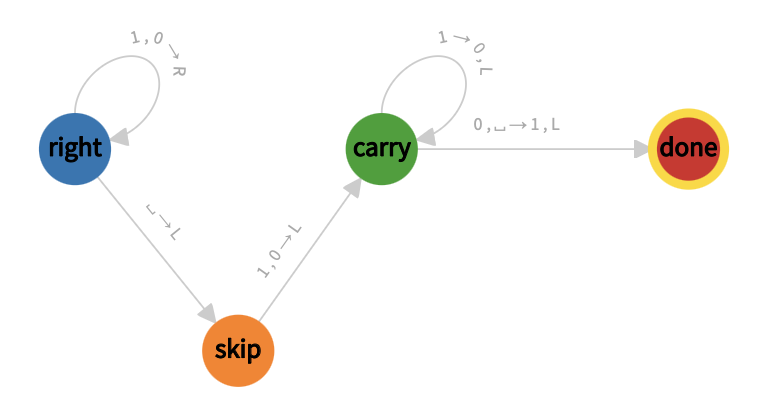
\includegraphics[width=0.7\linewidth]{add2.png}\\[1em]
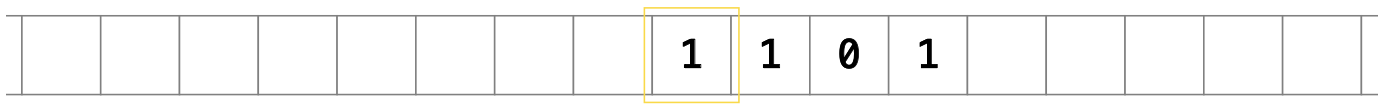
\includegraphics[width=0.95\linewidth]{add2_tape.png}
\end{center}

For example, on input \texttt{1011} (eleven) the machine scans right to the blank, steps left onto the final \texttt{1}, steps left again onto \texttt{1} in state \texttt{carry}, writes \texttt{0} and moves left, reads \texttt{0}, writes \texttt{1} and stops in \texttt{done}.
The tape now reads \texttt{1101} (thirteen).
On input \texttt{1} the carry runs into the blank to the left and writes a \texttt{1} there, giving \texttt{11} (three).

\qpage{Q5.2 Turing machines (b)}

\textbf{Idea.}
Repeatedly cross off two $0$'s from the left and one $1$ from the left end of the $1$'s.
Crossed-off $0$'s are overwritten with $x$ and crossed-off $1$'s with $y$.
The very first $0$ is overwritten with $\$$ instead of $x$ so that the head can find the left end of the tape when it returns.
If a round cannot find its two $0$'s and one $1$ in the right order, reject.
If the head scans the whole tape and finds only crossed-off symbols, accept.

Tape alphabet $\Gamma = \set{0, 1, x, y, \$, \sqcup}$, input alphabet $\set{0,1}$.
Edge labels are \emph{read} $\to$ \emph{write}, \emph{move}; when the write is omitted the symbol is left unchanged.
Every transition not drawn goes to $q_{\text{rej}}$ (moving right, say).

\begin{center}
\begin{tikzpicture}[auto,font=\small,>=Stealth]
  \node[state,initial above]     (qs)  at (3,2.4)   {$q_s$};
  \node[state]                   (q0)  at (0,0)     {$q_0$};
  \node[state]                   (q1)  at (3,0)     {$q_1$};
  \node[state]                   (q2)  at (6,0)     {$q_2$};
  \node[state]                   (q4)  at (0,-2.6)  {$q_4$};
  \node[state]                   (q3)  at (6,-2.6)  {$q_3$};
  \node[state,accepting]         (acc) at (-3.2,-1.3) {$q_{\text{acc}}$};
  \node[state,accepting]         (rej) at (9.2,-1.3)  {$q_{\text{rej}}$};
  \path[->]
    (qs) edge node[swap] {$0 \to \$,\mathrm{R}$} (q1)
    (qs) edge[bend right=40] node[swap,pos=0.25] {$\sqcup \to \mathrm{R}$} (acc)
    (qs) edge[bend left=28]  node[pos=0.35] {$1 \to \mathrm{R}$} (rej)
    (q0) edge[loop above] node {$x \to \mathrm{R}$} (q0)
    (q0) edge node {$0 \to x,\mathrm{R}$} (q1)
    (q0) edge node[swap] {$y \to \mathrm{R}$} (q4)
    (q0) edge node[swap] {$\sqcup \to \mathrm{R}$} (acc)
    (q1) edge node {$0 \to x,\mathrm{R}$} (q2)
    (q2) edge[loop above] node {$0,y \to \mathrm{R}$} (q2)
    (q2) edge node {$1 \to y,\mathrm{L}$} (q3)
    (q3) edge[loop below] node {$0,x,y \to \mathrm{L}$} (q3)
    (q3) edge node[pos=0.35] {$\$ \to \mathrm{R}$} (q0)
    (q4) edge[loop below] node {$y \to \mathrm{R}$} (q4)
    (q4) edge node {$\sqcup \to \mathrm{R}$} (acc);
\end{tikzpicture}
\end{center}

In words, the states mean:
\begin{itemize}
  \item $q_s$ (start): if the tape is empty, accept ($k = 0$); if it starts with $0$, mark it with $\$$ and look for the second $0$; if it starts with $1$, reject.
  \item $q_0$: skip crossed-off $0$'s ($x$) and find the next uncrossed $0$. If instead we see $y$, all $0$'s are used up, so go to $q_4$ to check that nothing but crossed-off $1$'s remain. If we see a blank, everything has been matched: accept. Seeing a $1$ means an unmatched $1$ with no $0$'s left: reject.
  \item $q_1$: the second $0$ of this round must come immediately; cross it off. Anything else means the number of $0$'s is odd or the string is out of order: reject.
  \item $q_2$: move right over the remaining $0$'s and already-crossed $1$'s ($y$) to the first uncrossed $1$, cross it off, and turn around. A blank here means there are not enough $1$'s: reject.
  \item $q_3$: move left back to the $\$$ marker, then start the next round in $q_0$.
  \item $q_4$: after the last $0$ was used, the rest of the tape must consist only of $y$'s up to the blank; then accept. Any $0$ or $1$ here means a leftover or out-of-order symbol: reject.
\end{itemize}
Each round removes exactly two $0$'s and one $1$, the $0$'s are always taken from the left and the $1$ from the left end of the $1$'s, and the machine only accepts when every symbol has been crossed off with the tape in the form $\$\,x^{*}\,y^{*}$.
So it accepts exactly the strings $0^{2k}1^k$, and it halts on every input because every round moves the head strictly further into the input.

\qpage{Q6.1 Decidability (a)}

Let $L = \set{\ell_1, \ldots, \ell_n}$ be a finite language.
The strings $\ell_1, \ldots, \ell_n$ are fixed, so they can be written directly into the algorithm.

\begin{algorithmic}[1]
  \Require{A string $x$}
  \Ensure{accept if $x \in L$, reject otherwise}
  \Function{DecideFinite}{$x$}
    \For{$i = 1, \dots, n$}
      \If{$x = \ell_i$} \Comment{compare character by character}
        \State \Return accept
      \EndIf
    \EndFor
    \State \Return reject
  \EndFunction
\end{algorithmic}

\textbf{It always halts.}
The loop runs at most $n$ times, and $n$ is a fixed constant that does not depend on $x$.
Each iteration compares two finite strings, which takes at most $\max(\abs{x}, \abs{\ell_i}) + 1$ steps.
So the algorithm halts on every input.

\textbf{It is correct.}
If $x \in L$, then $x = \ell_i$ for some $i$, so the loop reaches that $i$ (or an earlier match) and returns accept.
If $x \notin L$, then $x \ne \ell_i$ for every $i$, so no iteration returns, and the algorithm returns reject after the loop.
So the algorithm accepts exactly the strings in $L$.

Since there is an algorithm that halts on every input and returns the right answer, and every algorithm can be implemented by a Turing machine, $L$ is decidable.
(The case $n = 0$, the empty language, is also covered: the loop body never runs and the algorithm always rejects.)

\qpage{Q6.2 Decidability (b)}

Since $L_1, L_2, L_3$ are decidable, there are algorithms $D_1, D_2, D_3$ that halt on every input and satisfy $D_i(x) = \text{accept}$ if and only if $x \in L_i$.
I use them as subroutines.

\begin{algorithmic}[1]
  \Require{A string $x$}
  \Ensure{accept if $x \in (L_1 \setminus L_2) \cup L_3$, reject otherwise}
  \Function{DecideL}{$x$}
    \If{$D_3(x) = \text{accept}$}
      \State \Return accept
    \EndIf
    \If{$D_1(x) = \text{accept}$ \textbf{and} $D_2(x) = \text{reject}$}
      \State \Return accept
    \EndIf
    \State \Return reject
  \EndFunction
\end{algorithmic}

\textbf{It always halts.}
The algorithm makes at most three calls, to $D_3$, $D_1$, and $D_2$, each of which halts on every input because the $L_i$ are decidable.
Everything else is a constant number of comparisons.
So \algo{DecideL} halts on every input.

\textbf{It is correct.}
Unfold the definition: $x \in L$ if and only if $x \in L_3$, or ($x \in L_1$ and $x \notin L_2$).
\begin{itemize}
  \item If $x \in L$ and $x \in L_3$, then $D_3(x)$ accepts, so the algorithm accepts at the first \textbf{if}.
  \item If $x \in L$ and $x \notin L_3$, then $x \in L_1$ and $x \notin L_2$, so $D_1(x)$ accepts and $D_2(x)$ rejects, and the algorithm accepts at the second \textbf{if}.
  \item If $x \notin L$, then $x \notin L_3$, so the first \textbf{if} does not fire, and it is not the case that ($x \in L_1$ and $x \notin L_2$), so the second \textbf{if} does not fire either. The algorithm reaches the last line and rejects.
\end{itemize}
So \algo{DecideL} accepts exactly the strings in $L$, and $L$ is decidable.

\qpage{Q7.1 Pac-Man's journey (a)}

Pac-Man's final position is $(\#\mathtt{R} - \#\mathtt{L},\ \#\mathtt{U} - \#\mathtt{D})$.
Whether a coordinate is even depends only on its value mod $2$, and $\#\mathtt{R} - \#\mathtt{L} \equiv \#\mathtt{R} + \#\mathtt{L} \pmod 2$.
So the DFA only needs to track the parity of the $x$-coordinate and the parity of the $y$-coordinate.
Each $\mathtt{L}$ or $\mathtt{R}$ flips the $x$-parity, and each $\mathtt{U}$ or $\mathtt{D}$ flips the $y$-parity.

States are pairs $(p_x, p_y) \in \set{0,1}^2$, where $p_x$ is the $x$-coordinate mod $2$ and $p_y$ is the $y$-coordinate mod $2$.

\begin{center}
\begin{tikzpicture}[node distance=3.2cm,auto]
  \node[state,initial,accepting]       (00) {$(0,0)$};
  \node[state,right=of 00]             (10) {$(1,0)$};
  \node[state,below=2.4cm of 00]       (01) {$(0,1)$};
  \node[state,below=2.4cm of 10]       (11) {$(1,1)$};
  \path[->]
    (00) edge[bend left=15] node {$\mathtt{L},\mathtt{R}$} (10)
    (10) edge[bend left=15] node {$\mathtt{L},\mathtt{R}$} (00)
    (01) edge[bend left=15] node {$\mathtt{L},\mathtt{R}$} (11)
    (11) edge[bend left=15] node {$\mathtt{L},\mathtt{R}$} (01)
    (00) edge[bend left=15] node {$\mathtt{U},\mathtt{D}$} (01)
    (01) edge[bend left=15] node {$\mathtt{U},\mathtt{D}$} (00)
    (10) edge[bend left=15] node {$\mathtt{U},\mathtt{D}$} (11)
    (11) edge[bend left=15] node {$\mathtt{U},\mathtt{D}$} (10);
\end{tikzpicture}
\end{center}

Formally: $\Sigma = \set{\mathtt{L},\mathtt{R},\mathtt{U},\mathtt{D}}$, $Q = \set{0,1}^2$, start state $(0,0)$, $F = \set{(0,0)}$, and
\[
  \delta\big((p_x,p_y), \mathtt{L}\big) = \delta\big((p_x,p_y), \mathtt{R}\big) = (1-p_x,\ p_y), \qquad
  \delta\big((p_x,p_y), \mathtt{U}\big) = \delta\big((p_x,p_y), \mathtt{D}\big) = (p_x,\ 1-p_y).
\]

\textbf{Justification.}
By induction on the length of the command string $s$, after reading $s$ the DFA is in state $(x \bmod 2,\ y \bmod 2)$ where $(x,y)$ is Pac-Man's position after executing $s$.
This is true for $s = \varepsilon$ since Pac-Man starts at $(0,0)$ and so does the DFA.
Appending one command changes exactly one coordinate by $\pm 1$, which flips that coordinate's parity and leaves the other alone, and that is exactly what the corresponding transition does.
Pac-Man ends at an even position exactly when both parities are $0$, i.e., when the DFA ends in $(0,0)$, the only accepting state.

\qpage{Q7.2 Pac-Man's journey (b)}

Let $L_{\text{home}}$ be the set of command strings after which Pac-Man is back at $(0,0)$.
Suppose, for contradiction, that some DFA $M$ with $p$ states decides $L_{\text{home}}$.

Consider the $p+1$ strings $\mathtt{R}^0, \mathtt{R}^1, \mathtt{R}^2, \ldots, \mathtt{R}^{p}$.
Since $M$ has only $p$ states, by the pigeonhole principle two of these strings, say $\mathtt{R}^i$ and $\mathtt{R}^j$ with $0 \le i < j \le p$, leave $M$ in the same state $q$.

A DFA's future behavior depends only on its current state and the remaining input.
So for any string $z$, the strings $\mathtt{R}^i z$ and $\mathtt{R}^j z$ end in the same state, and $M$ either accepts both or rejects both.

Now take $z = \mathtt{L}^i$.
\begin{itemize}
  \item $\mathtt{R}^i \mathtt{L}^i$ moves Pac-Man $i$ steps right and then $i$ steps left, ending at $(0,0)$. So it is in $L_{\text{home}}$, and $M$ must accept it.
  \item $\mathtt{R}^j \mathtt{L}^i$ ends at $(j - i, 0)$ with $j - i \ge 1$, which is not the origin. So it is not in $L_{\text{home}}$, and $M$ must reject it.
\end{itemize}
But $M$ treats both strings the same way, so it gives the wrong answer on one of them.
This contradicts the assumption that $M$ decides $L_{\text{home}}$.
Since $p$ was arbitrary, no DFA decides $L_{\text{home}}$.

Intuitively, a DFA has a fixed finite memory, but to know whether Pac-Man will get back home it must remember how far right it has gone, which can be any integer.

\qpage{Q7.3 Pac-Man's journey (c)}

\begin{algorithmic}[1]
  \Require{A command string $s = s_1 s_2 \cdots s_n$ over $\set{\mathtt{L},\mathtt{R},\mathtt{U},\mathtt{D}}$}
  \Ensure{accept if Pac-Man ends at $(0,0)$ after executing $s$, reject otherwise}
  \Function{BackHome}{$s$}
    \State $x \gets 0$, $y \gets 0$
    \For{$i = 1, \dots, n$}
      \If{$s_i = \mathtt{L}$} $x \gets x - 1$
      \ElsIf{$s_i = \mathtt{R}$} $x \gets x + 1$
      \ElsIf{$s_i = \mathtt{U}$} $y \gets y + 1$
      \Else{} $y \gets y - 1$ \Comment{$s_i = \mathtt{D}$}
      \EndIf
    \EndFor
    \If{$x = 0$ \textbf{and} $y = 0$} \Return accept
    \Else{} \Return reject
    \EndIf
  \EndFunction
\end{algorithmic}

\textbf{Correctness.}
Claim: after the $i$-th iteration of the loop, $(x,y)$ equals Pac-Man's position after executing the first $i$ commands $s_1 \cdots s_i$.
For $i = 0$ both are $(0,0)$, the starting position.
If the claim holds after iteration $i-1$, then the $i$-th iteration changes $(x,y)$ by exactly the unit move that command $s_i$ makes (left decreases $x$, right increases $x$, up increases $y$, down decreases $y$), so the claim holds after iteration $i$.
By induction, after the loop $(x,y)$ is Pac-Man's final position, and the algorithm accepts exactly when that position is $(0,0)$.

The loop runs $n$ times and the algorithm clearly halts, so this is a decider for $L_{\text{home}}$.
The difference from a DFA is that the counters $x$ and $y$ can grow without bound, which a finite set of states cannot do.

\qpage{Q8.3 Decision problems and languages (c)}

``Given an array $S$ of integers, are all its elements distinct?''

\begin{enumerate}[(i)]
  \item The elements can be negative, so I add a minus sign to the alphabet from the sorted-array example:
  $\Sigma = \set{\mathtt{0}, \ldots, \mathtt{9}, \mathtt{-}, \mathtt{[}, \mathtt{,}, \mathtt{]}}$.

  \item Encoding: write the elements in base $10$ (with a leading $\mathtt{-}$ for negative numbers), separated by commas and enclosed in brackets.
  For example, the array $S$ with entries five, negative twelve, zero, and five has $\inner{S} = \mathtt{[5,-12,0,5]}$.

  \item For $S = (a_1, \ldots, a_n)$, element $a_i$ takes $1 + \floor{\log_{10} \abs{a_i}}$ digits (one digit when $a_i = 0$), plus one more character if it is negative, so $\Theta(\log(\abs{a_i} + 2))$ characters.
  Add the two brackets and $n-1$ commas, which is $n+1$ characters.
  The total length is
  \[
    \abs{\inner{S}} = \Theta\Big(n + \sum_{i=1}^{n} \log(\abs{a_i} + 2)\Big).
  \]
  If every element has absolute value at most $M$, this is $O(n \log M)$.

  \item The language is
  \[
    L_{\text{distinct}} = \set{\inner{S} : S \text{ is an array of integers and } a_i \ne a_j \text{ for all } i \ne j}.
  \]
\end{enumerate}

\qpage{Q8.4 Decision problems and languages (d)}

``Is a given undirected graph complete?''

\begin{enumerate}[(i)]
  \item Number the vertices $1, \ldots, n$ and write numbers in base $10$.
  $\Sigma = \set{\mathtt{0}, \ldots, \mathtt{9}, \mathtt{(}, \mathtt{)}, \mathtt{,}, \mathtt{;}}$.

  \item Encoding: write the number of vertices $n$, then a semicolon, then the list of edges, each as a pair $\mathtt{(}u\mathtt{,}v\mathtt{)}$ of vertex numbers, separated by commas.
  For example, the triangle on three vertices has
  \[
    \inner{G} = \mathtt{3;(1,2),(1,3),(2,3)},
  \]
  and the path $1 - 2 - 3$ has $\inner{G} = \mathtt{3;(1,2),(2,3)}$.

  \item Let $G$ have $n$ vertices and $m$ edges.
  The vertex count takes $\Theta(\log n)$ digits.
  Each edge takes two vertex numbers of at most $1 + \floor{\log_{10} n}$ digits each, plus four punctuation characters, so $\Theta(\log n)$ characters (treating $\log 1$ as $1$ character).
  The total length is
  \[
    \abs{\inner{G}} = \Theta\big((m + 1) \log n\big).
  \]
  Since $m \le \binom{n}{2}$, this is $O(n^2 \log n)$ in the worst case.
  (An adjacency-matrix encoding over $\set{\mathtt 0, \mathtt 1, \mathtt ;}$ would have length $\Theta(n^2)$ instead.)

  \item The language is
  \[
    L_{\text{complete}} = \set{\inner{G} : G \text{ is a complete undirected graph}},
  \]
  where ``complete'' means that every two distinct vertices of $G$ are adjacent.
  Equivalently, if $G$ has $n$ vertices, its edge set is exactly $\set{(u,v) : 1 \le u < v \le n}$.
\end{enumerate}

\qpage{Q8.5 Decision problems and languages (e)}

``Does a given C++ program terminate when run on a given input?''

\begin{enumerate}[(i)]
  \item A C++ source file is a string of ASCII characters, and so is the program's input.
  I take $\Sigma$ to be the set of ASCII characters plus one extra separator symbol $\#$ that is not an ASCII character, so that it cannot appear inside the program or its input.

  \item Encoding: the input object is a pair (program $P$, input string $x$).
  Encode it as
  \[
    \inner{P, x} = \inner{P}\,\#\,\inner{x},
  \]
  where $\inner{P}$ is the source code of $P$ written out character by character, and $\inner{x}$ is the input string itself.
  For example, if $P$ is the program
  \texttt{int main()\{while(1);\}} and $x$ is the input \texttt{42}, then
  $\inner{P,x} = \texttt{int main()\{while(1);\}\#42}$.
  Because $\#$ occurs exactly once, the encoding can be split back into $P$ and $x$ unambiguously.

  \item The length is simply the length of the source code plus the length of the input plus one:
  \[
    \abs{\inner{P,x}} = \abs{P} + \abs{x} + 1 = \Theta(\abs{P} + \abs{x}).
  \]

  \item The language is
  \[
    L_{\text{halt}} = \set{\inner{P,x} : P \text{ is a valid C++ program and } P \text{ halts when run on input } x}.
  \]
  (This is the halting problem for C++ programs. It is a perfectly well-defined language, even though, as we will see, no algorithm decides it.)
\end{enumerate}

\qpage{Q9.1 Trophy testing (a, optional)}

\textbf{Method.}
Suppose I have $d$ drops left and both blocks intact.
Drop the first block from height $h = d$.
\begin{itemize}
  \item If it breaks, the LBH is one of $1, \ldots, d$.
  I have one block and $d-1$ drops left, so I test heights $1, 2, \ldots, d-1$ in order with the second block.
  The first height at which it breaks is the LBH; if it never breaks, the LBH is $d$.
  This never needs more than $d-1$ drops.
  \item If it does not break, the LBH is more than $d$.
  I still have two blocks and $d-1$ drops, so I recursively run the same strategy on the heights above $d$, i.e., the next drop is from height $d + (d-1)$, and so on.
\end{itemize}
In other words, the first-block drops are at heights $d,\ d+(d-1),\ d+(d-1)+(d-2), \ldots$, and when the first block breaks, the second block sweeps the gap below it one inch at a time.
After $d$ drops, every gap has been searched or the total height has been cleared.

\textbf{Recurrence.}
Let $n(d)$ be the largest $n$ for which $d$ drops and two blocks suffice to determine the LBH among the $n+1$ possibilities $\set{1, \ldots, n, \text{``more than } n\text{''}}$.
With $0$ drops nothing can be tested, so only one possibility can be handled: $n(0) = 0$.
With $d \ge 1$ drops, the first drop from height $d$ covers $d$ heights (the heights $1, \ldots, d$ in the break case), and the no-break case leaves a fresh $(d-1)$-drop problem that covers $n(d-1)$ further heights.
So
\[
  n(d) = d + n(d-1), \qquad n(0) = 0.
\]

\textbf{Closed form.}
Unrolling, $n(d) = d + (d-1) + \cdots + 1 + n(0)$, so
\[
  n(d) = \frac{d(d+1)}{2}.
\]
As a check: $n(1) = 1$ (drop from $1$: breaks means LBH $1$, otherwise ``more than $1$''), $n(2) = 3$, $n(3) = 6$, $n(4) = 10$.

\qpage{Q9.2 Trophy testing (b, optional)}

Let $N(d)$ be the largest $n$ that \emph{any} strategy with two blocks and at most $d$ drops can handle.
I show $N(d) \le d + N(d-1)$ with $N(0) = 0$, which gives $N(d) \le d(d+1)/2 = n(d)$ by the same unrolling as in part (a).

With $0$ drops there is no information, so only one possibility can be distinguished: $N(0) = 0$.

Now consider any strategy with $d \ge 1$ drops, and let $h$ be the height of its first drop.
The adversary (nature) can choose either outcome.
\begin{itemize}
  \item \textbf{If it breaks}, the LBH is in $\set{1, \ldots, h}$, and only one block remains.
  With one block, no height below $h$ can be skipped: if the strategy skipped some height $t < h$ and the block then broke at a higher height, it could not tell whether the LBH was $t$ or that higher height, and there are no blocks left to find out.
  So the strategy must drop from $1, 2, \ldots$ one at a time.
  With $d-1$ drops left it can check at most $d-1$ heights, which decides among at most $d$ possibilities ($1, \ldots, d-1$ and ``higher''), so $h \le d$.
  \item \textbf{If it does not break}, the LBH is more than $h$.
  The strategy now has two blocks and $d-1$ drops, so by definition of $N$ it can handle at most $N(d-1)$ heights above $h$.
\end{itemize}
Putting the two cases together, the strategy can handle at most $h + N(d-1) \le d + N(d-1)$ heights.
Since this holds for every strategy, $N(d) \le d + N(d-1)$, and so $N(d) \le d(d+1)/2 = n(d)$.
The strategy in part (a) achieves this bound, so it is optimal.

\end{document}
